% Geant4 Physics Manual Entry
%
% Use 'make' to run latex and generate the pdf file
%
% Doug Wright

\documentclass[11pt]{article}
%\usepackage{h4}
% Original Author: Doug Wright   September 9, 2003

%%%%%
%%%%% Load useful packages
%%%%%
\usepackage{graphicx} % \includegraphics needed for Figures
\usepackage{amsmath}  % enhance math modes
\usepackage{times}    % use Times Roman text font 
                      % instead of default Computer Modern Roman
\usepackage{mathptmx} % use Times Roman font in math mode
                      % need this if you use times.sty

%....set paper to USletter with 1in margins (default is A4)
%    this works great with pdflatex 
%    if you are using dvips or dvipdf you might need to run
%     texconfig dvips paper letter
%     texconfig xdvi us                 #....if you use xdvi

\usepackage{vmargin}
\setpapersize{USletter}
\setmarginsrb{1in}{1in}{1in}{1in}{0pt}{0mm}{0pt}{0mm}
\footskip=2\baselineskip   %....put page number in middle of footer

% LC version of fullpage.sty is out of date and does not give proper margins
% so copied the new version (from MacOSX) into reports/macros
%   /usr/share/texmf/tex/latex/misc/fullpage.sty  (1998)    BAD
%   /usr/share/texmf/tex/latex/preprint/fullpage.sty (1999) GOOD
%
%\usepackage{h4fullpage} % set paper to USletter and margins to 1in all around
%\headsep=2\baselineskip % otherwise headings run into the text at top of page

% Make sure that dvips and xdvi are using 8.5x11 (default is A4)
% Use 'texconfig dvips paper letter' to set the defaults to letter
%     'texconfig xdvi us'

%%%%%
%%%%% change title to include doc# and UCRL (if available)
%%%%%
\newcommand{\mytitle}[1]{
\title{ {\small \hfill \versionnum\\
                \hfill \ucrlnum\\}
        \bf #1}}

\newcommand{\version}[1]{\newcommand{\versionnum}{#1}}
\newcommand{\ucrl}[1]{\newcommand{\ucrlnum}{#1}}

%%%%%
%%%%% Figure macros
%%%%%
%%%%% \Figure{file}{caption}             % expects eps/file.eps
%%%%% \FigureH{hsize}{file}{caption}     % height=hsize e.g. 4in
%%%%% \FigureW{wsize}{file}{caption}     % width =wsize
%%%%% \FigureWfrac{wsize}{file}{caption} % width=wsize /linewidth
%%%%%
%%%%% Reference figure as, Figure~\ref{file}
%%%%%

\newcommand{\Figure}[2]      {\epsFigure{                   }{#1}{#2}}
\newcommand{\FigureH}[3]     {\epsFigure{ height=#1         }{#2}{#3}}
\newcommand{\FigureW}[3]     {\epsFigure{ width=#1          }{#2}{#3}}
\newcommand{\FigureWfrac}[3] {\epsFigure{ width=#1\linewidth}{#2}{#3}}

%%%%%
%%%%% \epsFigure{size}{file}{caption}
%%%%%
\newcommand{\epsFigure}[3]{
  \def\file@{eps/#2.eps}  %....look for files in subdir 'eps'
  \IfFileExists{\file@}    
    { \def\insert@{ \includegraphics[#1]{\file@}}} %....insert file if it exists
    { \def\insert@{ \framebox[5in]{\rule{0in}{3in}\file@}}}  %....otherwise make box with the filename
    \genericFigure{\insert@}{#2}{#3}
}

%%%%%
%%%%% \genericFigure{graphics_command}{label}{caption}
%%%%%
\newcommand{\genericFigure}[3]{
  \begin{figure}[hbt] \centering
  \mbox{#1}\\
  \mycaption{#3}{#2}
  \end{figure}}

\newcommand{\mycaption}[2]{\parbox{5in}{\caption{#1\label{#2}}}}

%%%%%
%%%%% Table macros
%%%%%
%%%%%          1       2      3       4
%%%%% \Table{label}{caption}{layout}{data}
%%%%%
%%%%% \Table{table1}{Event fractions for different candidate types}{|l|r|}{
%%%%% \hline
%%%%% Type      & Fraction (\%) \\ 
%%%%% IFR   & 35  \\
%%%%% ECAL  & 30  \\
%%%%% Total & 65  \\ 
%%%%% \hline
%%%%% }
%%%%%
\newcommand{\Table}[4]{
\begin{table}[bt]
\begin{center}
\caption{#2\label{#1}}\medskip
\begin{tabular}{#3}#4
\end{tabular}
\end{center}
\end{table}
}


\newcommand{\notgeant}[1]{}% exclude some things from the geant manual

%\ucrl{UCRL-AR-228518}

\begin{document}

\section{Fission with improved multiplicity sampling}

As an alternative to the fission model described in the previous
section there is a modified model that produces more accurate
multiplicity distributions for the emitted neutrons and gamma rays
from spontaneous and neutron-induced fission. This was motivated by
detailed statistical studies of fission chains in multiplying
media. This model is data-driven and incorporates all available
multiplicity measurements found in the literature. Empirical models
are employed whenever multiplicity data are not available.
Essentially no data are available for the correlations between the
neutrons and gammas, so this model samples these distributions
independently. By default, this model effectively scales the
multiplicity data to match the average multiplicity value
($\bar{\nu}$) found in the GEANT4 evaluated data library. Therefore,
only isotopes that have a measured $\bar{\nu}$ in the data library
will emit fission gammas or neutrons. At present the gammas and
neutrons are emitted isotropically. The data and empirical models are
described in detail in the following subsections.

%\section{Neutrons emitted by fission\label{neutrons}}

\subsection{Neutron number distribution}

Based on reasonable assumptions about the distribution of excitation
energy among fission fragments, Terrell~\cite{Terrell 1957} showed
that the probability P$_\nu$ of observing $\nu$ neutrons from fission
can be approximated by a Gaussian-like distribution
\begin{equation}
\sum_{n=0}^{\nu}P_n = \frac{1}{2\pi}\int_{-\infty}^{\frac{\nu-\bar{\nu} 
                    + \frac{1}{2}+b}{\sigma}}e^{-\frac{t^2}{2}dt}
\end{equation}
where $\bar{\nu}$ is the average number of neutrons, $\sigma$ (set to
1.079) is the width of the distribution, and $b$ is a small correction
factor ($b<0.01$) that ensures that the discrete probability
distribution has the correct average $\bar{\nu}$. This model is used
when no explicit multiplicity data are available.

\subsubsection*{Neutron-induced fission data}

Zucker and Holden~\cite{Zucker and Holden 1986} measured the neutron
multiplicity distributions for $^{235}$U, $^{238}$U, and $^{239}$Pu
(see Tables~\ref{Neutron number distribution for induced fission in
235U}-\ref{Neutron number distribution for induced fission in 239Pu}),
as a function of the incident neutron energy $E_n$ from 
zero through ten MeV in increments of one MeV.  Fig.~\ref{235U induced
fission 6MeV} shows the neutron number distribution for induced
fission of $^{235}$U. Gwin, Spencer and Ingle~\cite{Gwin 1984}
measured the distribution at thermal energies for $^{235}$U. In
addition, there are many measurements of $\bar{\nu}$, the average
number of emitted neutrons, for many isotopes. Since there are multiple
methods for parameterizing the multiplicity data and 
renormalizing the overall distributions to agree with the specific measured
values of $\bar{\nu}$, we provide four options for generating 
neutron multiplicity distributions. 
\notgeant{These options are selected by the internal variable {\tt nudist}, default=3.}

\begin{table}[ht]
\footnotesize
\begin{center}
\begin{tabular}{|c|cccccccc|c|} \hline
$E_n$ & $\nu$=0 & 1 & 2 & 3 & 4 & 5 & 6 & 7 & $\bar{\nu}$ \\ \hline
0 & .0317223 & .1717071 & .3361991 & .3039695 & .1269459 & .0266793 & .0026322 & .0001449 & 2.4140000 \\
1 & .0237898 & .1555525 & .3216515 & .3150433 & .1444732 & .0356013 & .0034339 & .0004546 & 2.5236700 \\
2 & .0183989 & .1384891 & .3062123 & .3217566 & .1628673 & .0455972 & .0055694 & .0011093 & 2.6368200 \\
3 & .0141460 & .1194839 & .2883075 & .3266568 & .1836014 & .0569113 & .0089426 & .0019504 & 2.7623400 \\
4 & .0115208 & .1032624 & .2716849 & .3283426 & .2021206 & .0674456 & .0128924 & .0027307 & 2.8738400 \\
5 & .0078498 & .0802010 & .2456595 & .3308175 & .2291646 & .0836912 & .0187016 & .0039148 & 3.0386999 \\
6 & .0046272 & .0563321 & .2132296 & .3290407 & .2599806 & .1045974 & .0265604 & .0056322 & 3.2316099 \\
7 & .0024659 & .0360957 & .1788634 & .3210507 & .2892537 & .1282576 & .0360887 & .0079244 & 3.4272800 \\
8 & .0012702 & .0216090 & .1472227 & .3083032 & .3123950 & .1522540 & .0462449 & .0107009 & 3.6041900 \\
9 & .0007288 & .0134879 & .1231200 & .2949390 & .3258251 & .1731879 & .0551737 & .0135376 & 3.7395900 \\
10& .0004373 & .0080115 & .1002329 & .2779283 & .3342611 & .1966100 & .0650090 & .0175099 & 3.8749800 \\ \hline
\end{tabular}
\end{center}
\caption{Neutron number distribution for induced fission in $^{235}$U.}
\label{Neutron number distribution for induced fission in 235U}
\end{table}

\begin{table}[ht]
\footnotesize
\begin{center}
\begin{tabular}{|c|ccccccccc|c|} \hline
$E_n$ & $\nu$=0 & 1 & 2 & 3 & 4 & 5 & 6 & 7 & 8 & $\bar{\nu}$ \\ \hline
0 & .0396484 & .2529541 & .2939544 & .2644470 & .1111758 & .0312261 & .0059347 & .0005436 & .0001158 & 2.2753781 \\
1 & .0299076 & .2043215 & .2995886 & .2914889 & .1301480 & .0363119 & .0073638 & .0006947 & .0001751 & 2.4305631 \\
2 & .0226651 & .1624020 & .2957263 & .3119098 & .1528786 & .0434233 & .0097473 & .0009318 & .0003159 & 2.5857481 \\
3 & .0170253 & .1272992 & .2840540 & .3260192 & .1779579 & .0526575 & .0130997 & .0013467 & .0005405 & 2.7409331 \\
4 & .0124932 & .0984797 & .2661875 & .3344938 & .2040116 & .0640468 & .0173837 & .0020308 & .0008730 & 2.8961181 \\
5 & .0088167 & .0751744 & .2436570 & .3379711 & .2297901 & .0775971 & .0225619 & .0030689 & .0013626 & 3.0513031 \\
6 & .0058736 & .0565985 & .2179252 & .3368863 & .2541575 & .0933127 & .0286200 & .0045431 & .0031316 & 3.2064881 \\
7 & .0035997 & .0420460 & .1904095 & .3314575 & .2760413 & .1112075 & .0355683 & .0065387 & .0031316 & 3.3616731 \\
8 & .0019495 & .0309087 & .1625055 & .3217392 & .2943792 & .1313074 & .0434347 & .0091474 & .0046284 & 3.5168581 \\
9 & .0008767 & .0226587 & .1356058 & .3076919 & .3080816 & .1536446 & .0522549 & .0124682 & .0067176 & 3.6720432 \\
10& .0003271 & .0168184 & .1111114 & .2892434 & .3160166 & .1782484 & .0620617 & .0166066 & .0095665 & 3.8272281 \\ \hline
\end{tabular}
\end{center}
\caption{Neutron number distribution for induced fission in $^{238}$U.}
\label{Neutron number distribution for induced fission in 238U}
\end{table}

\begin{table}[ht]
\footnotesize
\begin{center}
\begin{tabular}{|c|ccccccccc|c|} \hline
$E_n$ & $\nu$=0 & 1 & 2 & 3 & 4 & 5 & 6 & 7 & 8 & $\bar{\nu}$ \\ \hline
0 & .0108826 & .0994916 & .2748898 & .3269196 & .2046061 & .0726834 & .0097282 & .0006301 & .0001685 & 2.8760000 \\
1 & .0084842 & .0790030 & .2536175 & .3289870 & .2328111 & .0800161 & .0155581 & .0011760 & .0003469 & 3.0088800 \\
2 & .0062555 & .0611921 & .2265608 & .3260637 & .2588354 & .0956070 & .0224705 & .0025946 & .0005205 & 3.1628300 \\
3 & .0045860 & .0477879 & .1983002 & .3184667 & .2792811 & .1158950 & .0301128 & .0048471 & .0007233 & 3.3167800 \\
4 & .0032908 & .0374390 & .1704196 & .3071862 & .2948565 & .1392594 & .0386738 & .0078701 & .0010046 & 3.4707300 \\
5 & .0022750 & .0291416 & .1437645 & .2928006 & .3063902 & .1641647 & .0484343 & .0116151 & .0014149 & 3.6246800 \\
6 & .0014893 & .0222369 & .1190439 & .2756297 & .3144908 & .1892897 & .0597353 & .0160828 & .0029917 & 3.7786300 \\
7 & .0009061 & .0163528 & .0968110 & .2558524 & .3194566 & .2134888 & .0729739 & .0213339 & .0020017 & 3.9325800 \\
8 & .0004647 & .0113283 & .0775201 & .2335926 & .3213289 & .2356614 & .0886183 & .0274895 & .0039531 & 4.0865300 \\
9 & .0002800 & .0071460 & .0615577 & .2089810 & .3200121 & .2545846 & .1072344 & .0347255 & .0054786 & 4.2404900 \\
10& .0002064 & .0038856 & .0492548 & .1822078 & .3154159 & .2687282 & .1295143 & .0432654 & .0075217 & 4.3944400 \\ \hline
\end{tabular}
\end{center}
\caption{Neutron number distribution for induced fission in $^{239}$Pu.}
\label{Neutron number distribution for induced fission in 239Pu}
\end{table}

\begin{figure}[ht]
\begin{center}
\includegraphics[scale=0.4, angle=-90]{eps/U235_6MeV_nudist.ps}
\end{center}
\caption{Induced fission in $^{235}$U, incident neutron energy = 6MeV}
\label{235U induced fission 6MeV}
\end{figure}

The first option\notgeant{ ({\tt nudist=0})} uses a fit to the Zucker
and Holden data \cite{Zucker and Holden 1986} by
Valentine~\cite{Valentine 1996}~\cite{Valentine 2000}. Valentine
expressed the P$_{\nu}$'s (for $\nu=0$, ..., 8) as 5$^{th}$ order
polynomials in $E_n$, the incident neutron energy. These functions 
P$_{\nu}(E_n)$ are used to sample the neutron multiplicity for 
$E_n$ in the range 0 to 10 MeV.  When $E_n$ is greater than 10 MeV, 
$E_n$=10 MeV is used to generate P$_{\nu}$.

In addition to using the Zucker and Holden data above for incident
neutron energies $E_n$ above 1 MeV, the second
option\notgeant{ ({\tt nudist=1})} also uses the Gwin, Spencer and
Ingle data~\cite{Gwin 1984} for $^{235}$U at thermal energies (0 MeV) 
to generate P$_{\nu}(E_n)$ polynomials. As in the first option, when
$E_n$ is greater than 10 MeV, $E_n$=10 MeV is used to generate
P$_{\nu}$.

The third option\notgeant{ ({\tt nudist=2})} implements an alternative
polynomial fit from Valentine ~\cite{Valentine 2000} of  P$_{\nu}$
as a function of $\bar{\nu}$ instead of $E_n$, following the suggestion 
of Frehaut~\cite{Frehaut 1988}.
%
%{\it"A unique
%relationship P$_{\nu}(\bar{\nu})$ can sufficiently
%well capture the multiplicity distributions of a number of major
%isotopes. This distribution is expressed as a function of the average
%number of neutrons emitted $\bar{\nu}$.}" 
%
When a neutron induces a fission, the algorithm converts the incident
neutron energy $E_n$ into $\bar{\nu}$ using conversion tables
(typically ENDF/EDNL), generates the P$_{\nu}$ distributions for that
value of $\bar{\nu}$, and then samples the P$_{\nu}$ distributions to
determine $\nu$. The least-square fits to the $^{235}$U data are used
for both $^{235}$U and $^{233}$U neutron induced fission, the fits to
$^{238}$U are used for $^{232}$U, $^{234}$U, $^{236}$U and $^{238}$U, while the
fits to $^{239}$Pu are used for $^{239}$Pu and $^{241}$Pu. Data comes from
Zucker and Holden. For $^{235}$U, data comes from Zucker and Holden 
for $E_n$ greater than 1 MeV, and Gwin, Spencer and
Ingle for 0 MeV. The fits are only used when $\bar{\nu}$ is in the 
range of the $\bar{\nu}$'s for the tabulated data. Otherwise, 
Terrell's approximation is used.

The fourth option, which is the default\notgeant{ ({\tt nudist=3})},
is similar to the third option except that the P$_{\nu}$ distributions
are not functions of $\bar{\nu}$, but are left intact as multiplicity
distributions for the data listed in Gwin, Spencer and
Ingle, and for the data listed in Zucker and
Holden. The multiplicity distribution P$_{\nu}$ from which the number
of neutrons will be sampled is selected based on the value of
$\bar{\nu}$ for a given induced fission event.  For instance, if
P$_{\nu}(1 MeV)$ has $\bar{\nu}=2.4$, P$_{\nu}(2 MeV)$ has
$\bar{\nu}=2.6$, and $\bar{\nu}$ is 2.45 at the energy of the incident
fission-inducing neutron (this value $\bar{\nu}$ comes typically from
cross-section data libraries such and ENDF/ENDL), the probability of
sampling the number of neutrons ${\nu}$ from P$_{\nu}(1 MeV)$ and
P$_{\nu}(2 MeV)$ will be 25\% and 75\%, respectively. This technique
is only used when $\bar{\nu}$ is in the range of the $\bar{\nu}$'s for
the tabulated data. Otherwise, Terrell's approximation is used.  This
last way of computing ${\nu}$ has several advantages: first, the data
as listed in the original papers is used exactly, as opposed to
approximated by low-ordered polynomials least-square fitting the
original data. Second, the data from the Gwin, Spencer and
Ingle paper, and the data from the Zucker and Holden paper is
entered as-is as a table in the code, and can easily be checked and
maintained if necessary by the application developer. Third the method
provides a simple and statistically correct mechanism of sampling the
data tables. \notgeant{The fission module behaves in this
manner when the 'nudist' option is set to 3, which is also the default
behavior.}

\subsubsection*{Spontaneous fission data}

For $^{252}$Cf, the fission module can be set to use either the
measurements by Spencer~\cite{Spencer 1982}\notgeant{ ({\tt ndist=0})},
which is the default,
or Boldeman~\cite{Boldeman 1985}\notgeant{ ({\tt ndist=1})}.

For $^{238}$U, $^{238}$Pu, $^{240}$Pu, $^{242}$Pu, $^{242}$Cm,
$^{244}$Cm, the probability distribution data comes from Holden and
Zucker~\cite{Holden and Zucker BNL}. The measured data is summarized
in Table~\ref{Neutron number distribution for spontaneous fission}.

\begin{table}[ht]
\footnotesize
\begin{center}
\begin{tabular}{|c|cccccccccc|} \hline
isotope & $\nu$=0 & 1 & 2 & 3 & 4 & 5 & 6 & 7 & 8 & 9 \\ \hline
$^{238}$U & .0481677 & .2485215 & .4253044 & .2284094 & .0423438 & .0072533 & 0 & 0 & 0 & 0 \\
$^{238}$Pu & .0540647 & .2053880 & .3802279 & .2248483 & .1078646 & .0276366 & 0 & 0 & 0 & 0 \\
$^{242}$Pu & .0679423 & .2293159 & .3341228 & .2475507 & .0996922 & .0182398 & .0031364 & 0 & 0 & 0 \\
$^{242}$Cm & .0212550 & .1467407 & .3267531 & .3268277 & .1375090 & .0373815 & .0025912 & .0007551 & .0001867 & 0 \\
$^{244}$Cm & .0150050 & .1161725 & .2998427 & .3331614 & .1837748 & .0429780 & .0087914 & .0002744 & 0 & 0 \\
$^{252}$Cf~\cite{Spencer 1982} & .00211 & .02467 & .12290 & .27144 & .30763 & .18770 & .06770 & .01406 & .00167 & .0001 \\
$^{252}$Cf~\cite{Boldeman 1985} & .00209 & .02621 & .12620 & .27520 & .30180 & .18460 & .06680 & .01500& .00210 & 0 \\ \hline
\end{tabular}
\end{center}
\caption{Neutron number distribution for spontaneous fission.}
\label{Neutron number distribution for spontaneous fission}
\end{table}

If no full multiplicity distribution data exists, the fission module
uses Terrell~\cite{Terrell 1957}'s approximation with $\bar{\nu}$ from
Ensslin~\cite{Ensslin 1998}.  Ensslin has $\bar{\nu}$ data for the
isotopes in table~\ref{Nubar for spontaneous fission}.

\begin{table}[ht]
\footnotesize
\begin{center}
\begin{tabular}{|c|c|} \hline
isotope & $\bar{\nu}$ \\ \hline
$^{232}$Th & 2.14 \\
$^{232}$U  & 1.71\\
$^{233}$U  & 1.76\\
$^{234}$U  & 1.81\\
$^{235}$U  & 1.86\\
$^{236}$U  & 1.91\\
$^{238}$U  & 2.01\\
$^{237}$Np & 2.05\\
$^{238}$Pu & 2.21\\
$^{239}$Pu & 2.16\\
$^{240}$Pu & 2.156\\
$^{241}$Pu & 2.25\\
$^{242}$Pu & 2.145\\
$^{241}$Am & 3.22\\
$^{242}$Cm & 2.54\\
$^{244}$Cm & 2.72\\
$^{249}$Bk & 3.40\\
$^{252}$Cf & 3.757\\ \hline
\end{tabular}
\end{center}
\caption{Average number of neutrons per spontaneous fission.}
\label{Nubar for spontaneous fission}
\end{table}

\subsection{Neutron energy distribution}

All of the fission spectra in the Evaluated Nuclear Data Library,
ENDL~\cite{ENDL 1975} are defined by a simple analytical function, a
Watt spectrum defined as

\begin{equation}
W(a,b,E') = Ce^{-aE'}sinh(\sqrt{bE'})
\end{equation}

where $C=\sqrt{\pi\frac{b}{4a}}\frac{e^{\frac{b}{4a}}}{a}$, and E' is the secondary neutron energy.
The Watt spectrum for $^{235}$U and an incident neutron energy of 6 MeV is shown in Fig.~\ref{Watt spectrum for U235}.

\begin{figure}[ht]
\begin{center}
\includegraphics[scale=0.4, angle=-90]{eps/Wattspectrum_U235_6MeV.ps}
\end{center}
\caption{Watt spectrum for $^{235}$U and an incident neutron energy of 6 MeV.}
\label{Watt spectrum for U235}
\end{figure}

The coefficients a and b vary weakly from one isotope to another and
also vary weakly with the incident neutron energy.  In the fission
module, b is set identical to 1.0, and a is parametrized as a simple
function of the incident neutron energy, as implemented in
TART~\cite{TART 2003, Cullen 2004}.  The fissioning isotope and
incident neutron energy determine the value of a, and the energy E' of
the secondary neutron emitted is sampled using the Los Alamos' Monte
Carlo sampler attributed to Mal Kalos~\cite{Everett 1983}.

The Watt spectrum is used for all isotopes except $^{252}$Cf, for which a
special treatment summarized by Valentine~\cite{Valentine 2000} is
applied.  The neutron spectrum for $^{252}$Cf is sampled from
the Mannhart~\cite{Mannhart 1987} corrected Maxwellian distribution, 
the Madland and Nix~\cite{Madland 1984}
or the Watt fission spectra from
Froehner~\cite{Froehner 1990}. 
\notgeant{These options are selected by the internal variable {\tt neng=0(default),1,2} respectively.} The Mannhart distribution is used by default.

%\section{Gammas emitted by fission\label{gammas}}

\subsection{Gamma-ray number distribution}

The fission module uses Brunson~\cite{Brunson 1982}'s double Poisson
model for the spontaneous fission gamma ray multiplicity of $^{252}$Cf
(see Fig.~\ref{Fission gamma-ray multiplicity for 252Cf}).

\begin{equation}
\Pi(G)=0.682\frac{7.20^Ge^{-7.20}}{G!}+0.318\frac{10.71^Ge^{-10.72}}{G!}
\end{equation}

where $G$ is the gamma ray multiplicity.
\begin{figure}[ht]
\begin{center}
\includegraphics[scale=0.4, angle=-90]{eps/Cf252_nugdist.ps}
\end{center}
\caption{Fission gamma-ray multiplicity for $^{252}$Cf.}
\label{Fission gamma-ray multiplicity for 252Cf}
\end{figure}

The prompt gamma ray multiplicity ranges from 0 to 20 gama rays per
fission with an average of 8.32 gamma rays per fission.  This model is
a fit to experimental data measured by Brunson himself.

For other isotopes, there is no data available for the multiplicity of
prompt gamma rays.  Valentine~\cite{Valentine 2001} used an
approximation that was adopted by the fission module.  The probability
of emitting $G$ fission gamma rays obeys the negative binomial
distribution:

\begin{equation}
\Pi(G)=\left(\begin{array}{c} \alpha+G-1 \\ G \end{array} \right) p^G(1-p)^G
\end{equation}

where the parameter $p$ can be written as
$p=\frac{\alpha}{\alpha+\bar{G}}$, $\alpha$ is approximately 26 and
$\bar{G}$ is the average number of gamma rays per fission.  $\bar{G}$
is approximated by

\begin{equation}
\bar{G} = \frac{E_t(\bar{\nu}, Z, A)}{\bar{E}}
\end{equation}

where $E_t(\bar{\nu}, Z,
A)=(2.51(\pm0.01)-1.13\cdot10^{-5}(\pm7.2\cdot10^{-8})Z^2\sqrt{A})\nu+4.0$
is the total prompt gamma ray energy, and $\bar{E} =
-1.33(\pm0.05)+119.6(\pm2.5)\frac{Z^{\frac{1}{3}}}{A}$ is the average
prompt gamma ray energy.  The multiplicity distribution for the
spontaneous fission of $^{238}$U is shown in Fig.~\ref{Fission
gamma-ray multiplicity for 238U}.

\begin{figure}[ht]
\begin{center}
\includegraphics[scale=0.4, angle=-90]{eps/U238_nugdist.ps}
\end{center}
\caption{Fission gamma-ray multiplicity for spontaneous fission of $^{238}$U.}
\label{Fission gamma-ray multiplicity for 238U}
\end{figure}

These multiplicity distributions are only estimates and are not
measured data.  The fission module uses this model for estimating the
number of gamma rays from both spontaneous and induced fission.

\subsection{Gamma-ray energy distribution}

The fission module implements Valentine's~\cite{Valentine 2000} model
for the energy spectra of fission gamma-rays.  The only measured
energy spectra for fission gamma-rays are for the spontaneous fission
of $^{252}$Cf and for the thermal-neutron-induced fission of $^{235}$U.
Both spectra are similar~\cite{Wagemans 1991}.  Because the $^{235}$U
measurements are more precise, this data will be used for the fission
gamma-ray spectrum.  The energy spectrum of the prompt fission gamma
rays is obtained from Maienschein's measurements~\cite{Maienschein
1958}~\cite{Goldstein 1959}:

\begin{equation}
N(E) = \left\{
\begin{array}{ll}
38.13 (E-0.085)e^{1.648E}&  E<0.3\ \mathrm{MeV} \\

26.8 e^{-2.30E}          &  0.3<E<1.0\ \mathrm{MeV}\\

 8.0 e^{-1.10E}          &  1.0<E<8.0\ \mathrm{MeV}
\end{array}
\right.
\end{equation}

This probability function is shown in Fig.~\ref{Fission gamma-ray
spectrum for 235U}.  Because gamma ray energy spectra are not
available, the spectrum above is used for all isotopes, both for
spontaneous and induced fission.

\begin{figure}[ht]
\begin{center}
\includegraphics[scale=0.4, angle=-90]{eps/U235_gspectrum.ps}
\end{center}
\caption{Fission gamma-ray spectrum for $^{235}$U.}
\label{Fission gamma-ray spectrum for 235U}
\end{figure}




\subsection{Implementation}

For neutron induced fission, this model is intended to be used with
the low energy neutron interaction data libraries with class
\textit{G4Fisslib} specified in the physics list as the
\textit{G4HadronFissionProccess} instead of class
\textit{G4NeutronHPFission}.\notgeant{
Here is an example code snippet for registering this model in the physics 
list: \begin{verbatim}
    G4ProcessManager* pmanager = particle->GetProcessManager();
    G4String particleName = particle->GetParticleName();

    if (particleName == "gamma") {
      (...)
    } else if (particleName == "neutron") {
      (...)
      // Fission library model
      G4HadronFissionProcess *theFissionProcess = new G4HadronFissionProcess();
      G4FissLib* theFissionModel = new G4FissLib;
      theFissionProcess->RegisterMe(theFissionModel);
      pmanager->AddDiscreteProcess(theFissionProcess);
      (...)
    } else ...
\end{verbatim}
}
The constructor of \textit{G4FissLib}
does two things. First it reads the necessary fission cross-section
data in the file located in the directory specified by the environment
variable \textit{NeutronHPCrossSections}. It does this by initializing
one object of class \textit{G4NeutronHPChannel} per isotope present in
the geometry. Second, it registers an instance of
\textit{G4FissionLibrary} for each isotope as the model for that
reaction/channel. When Geant4 tracks a neutron to a reaction site and
the fission library process is selected among all other process for
neutron reactions, the method \textit{G4FissLib::ApplyYourself} is
called, and one of the fissionable isotopes present at the reaction
site is selected. This method in turn calls
\textit{G4NeutronHPChannel::ApplyYourself} which calls
\textit{G4FissionLibrary::ApplyYourself}, where the induced neutrons
and gamma-rays are emitted by sampling the fission library.

For spontaneous fission the user must provide classes {\it
PrimaryGeneratorAction}, {\it MultipleSource}, {\it
MultipleSourceMessenger}, {\it SingleSource}, {\it SponFissIsotope} to
generate spontaneous fission neutrons and gammas. Examples of these
classes can be downloaded from \httpnuclear. Spontaneous fissions are
generated in the {\it PrimaryGeneratorAction} class.
The spontaneous fission
source needs to be described in terms of geometry, isotopic
composition and fission strength. Once this information is given, the
constructor creates as many spontaneous fission isotopes of class {\it
SponFissIsotope} as specified, and adds them to the source of class
{\it MultipleSource}. When Geant needs to generate particles, it calls
the method {\it PrimaryGeneratorAction::GeneratePrimaries}, which
first sets the time of the next fission based on the fission rates
entered in the constructor, and then calls the method {\it
MultipleSource::GeneratePrimaryVertex} which determines which one of
the spontaneous fission isotopes will fission. This method in turn
calls the method {\it SponFissIsotope::GeneratePrimaryVertex} for the
chosen isotope. It is in this method that the neutrons and photons
sampled from the fission library are added to the stack of secondary
particles.  Sources other than spontaneous fission isotopes can be
added to the source of class {\it MultipleSource}. For instance, a
background term emitting a large number of background gamma-rays can
be added, as long as it derives from the class {\it SingleSource}. The
intensity of that source would be set the same way as for the
spontaneous fission isotope sources.

Different sampling methods can be selected by calling the following functions.
\subsection*{void setnudist\_(int *nudist)
\label{setnudist}}

This selects the data to be sampled for the neutron number
distributions for neutron or photon induced fission. If there is no data
available, then in all cases the Terrell approximation is used.
The argument \textit{nudist} can take 3 values:

\begin{tabbing}

\indent 0 \hspace*{.55in} \= \parbox[t]{5.5in}{ Use the fit 
to the Zucker and Holden tabulated P$_\nu$ distributions as a function
of energy for $^{235}$U, $^{238}$U and $^{239}$Pu.}\\

\indent 1 \> \parbox[t]{5.5in}{Use fits to the Zucker and Holden tabulated 
P$_\nu$  distribution as a function of energy for $^{238}$U and 
 $^{239}$Pu, and a fit to the Zucker and Holden data as well as 
the Gwin, Spencer and Ingle data (at thermal 
 energies) as a function of energy for $^{235}$U.}\\

\indent 2 \> \parbox[t]{5.5in}{Use the fit to the Zucker and Holden 
tabulated P$_\nu$ distributions as a function of $\bar{\nu}$. The $^{238}$U 
fit is used for the $^{232}$U, $^{234}$U, 
$^{236}$U and $^{238}$U isotopes, the $^{235}$U fit for $^{233}$U 
and $^{235}$U, the $^{239}$Pu fit for 
$^{239}$Pu and $^{241}$Pu.}\\

\indent 3 (default) \> \parbox[t]{5.5in}{Use the discrete Zucker and Holden 
tabulated P$_\nu$ distributions and corresponding $\bar{\nu}$s. 
 Sampling
based on the incident neutron $\bar{\nu}$. The $^{238}$U data tables 
are used for the $^{232}$U, $^{234}$U, $^{236}$U 
 and $^{238}$U isotopes, the $^{235}$U data for $^{233}$U and 
$^{235}$U, the $^{239}$Pu data for $^{239}$Pu and $^{241}$Pu.}

\end{tabbing}

\subsection*{void setcf252\_(int *ndist, int *neng)}

This function is specific to the spontaneous fission of $^{252}$Cf. It
selects the data to be sampled for the neutron number and energy
distributions and takes the following arguments:

\begin{tabbing}
\indent ndist: \= Sample the number of neutrons \\
\indent \> 0 (default) \= 
from the tabulated data measured by Spencer \\
\indent \> 1 \> from 
Boldeman's data \\
\\
\indent neng: Sample the spontaneous fission 
neutron energy \\
\indent \> 0 (default)\> from Mannhart corrected  Maxwellian spectrum \\
\indent \> 1 \> from Madland-Nix theoretical spectrum \\
\indent \> 2 \> from the Froehner Watt spectrum \\
\end{tabbing}

\clearpage
\begin{thebibliography}{99}

\bibitem{Terrell 1957} J. Terrell, "Distributions of Fission Neutron
Numbers", \textit{Phys. Rev.} \textbf{108}, 783 (1957).

\bibitem{Cullen 2006} D.E. Cullen, "Sampling the Number of Neutrons
Emitted per Fission," UCRL-TR-222526, Lawrence Livermore National
Laboratory (2006).  

\bibitem{Zucker and Holden 1986} M.S. Zucker, N.E. Holden, "Energy
Dependence of Neutron Multiplicity P$_{\nu}$ in Fast-Neutron-Induced
Fission for $^{235,238}U$ and $^{239}Pu$," BNL-38491 (1986).

\bibitem{Gwin 1984} R. Gwin, R.R. Spencer,
R.W. Ingle, "Measurements of the Energy Dependence of Prompt Neutron
Emission from $^{233}U$, $^{235}U$, $^{239}Pu$, and $^{241}Pu$ for
$E_n=0.005$ to 10 eV Relative to Emission from Spontaneous Fission of
$^{252}$Cf," \textit{Nucl. Sci. Eng.}, \textbf{87}, 381 (1984).

\bibitem{Valentine 1996} T.E. Valentine, J.T. Mihalczo, "MCNP-DSP: A
Neutron and Gamma Ray Monte Carlo Calculation of Source-Driven
Noise-Measured Parameters ," \textit{Ann. of Nucl. Eng.}, \textbf{23},
16, p. 1271 (1996).

\bibitem{Valentine 2000} T.E. Valentine, "MCNP-DSP Users Manual,"
ORNL/TM-13334, R2, Oak Ridge National Laboratory (2000).

\bibitem{Frehaut 1988} J. Frehaut, "Neutron Multiplicity Distribution
in Fast Neutron-Induced Fission," \textit{Proc. of IAEA Consultant's
Meeting on Physics of Neutron Emission in Fission,}, Mito, Japan
(1988).  


\bibitem{Spencer 1982} R.R. Spencer, R. Gwin, R.W. Ingle, "A
measurement of the Average Number of Prompt Neutrons from Spontaneous
Fission of Californium-252," \textit{Nucl. Sci. Eng.} \textbf{80}, 603
(1982).  

\bibitem{Boldeman 1985} J.W. Boldeman, M.G. Hines, "Prompt
Neutron Emission Probabilities Following Spontaneous and Thermal
Neutron Fission," \textit{Nucl. Sci. Eng.}, \textbf{91}, 114 (1985).

\bibitem{Holden and Zucker BNL} N.E. Holden,
M.S. Zucker, "A Reevaluation of the Average Prompt Neutron Emission
Multiplicity ($\bar{\nu}$) Values from Fission of Uranium and
Transuranium Nuclides," BNL-NCS-35513, Brookhaven National
Laboratory).  

\bibitem{Ensslin 1998} N. Ensslin, W.C. Harker, M.S. Krick,
D.G. Langner, M.M. Pickrell, J.E. Stewart, "Application Guide to
Neutron Multiplicity Counting," LA-13422-M, Los Alamos National
Laboratory (1998).  

\bibitem{ENDL 1975} R.J. Howerton, et al, "The LLL
Evaluated Nuclear Data Library (ENDL): Evaluation Techniques, Reaction
Index, and Description of Individual Evaluations," UCRL-50400, V. 15,
Part A, Lawrence Livermore National Laboratory (1975).

\bibitem{TART 2003} D.E. Cullen, "TART 2002: A Couple
Neutron-Photon 3-D, Combinatorial Geometry, Time Dependent Monte-Carlo
Transport Code," UCRL-ID-126455, Rev. 4, Lawrence Livermore National
Laboratory (2003).  

\bibitem{Cullen 2004} D.E. Cullen, "Sampling ENDL Watt Fission
Spectra," UCRL-TR-203251, Lawrence Livermore National Laboratory
(2004).  

\bibitem{Everett 1983} C.J. Everett, E.D. Cashwell, "A Third
Monte Carlo Sampler," LA-9721-MS, Los Alamos National Laboratory
(1983).  


\bibitem{Mannhart 1987} W. Mannhart, "Evaluation
of the Cf-252 Fission Neutron Spectrum Between 0 MeV and 20 MeV,"
\textit{Proc. Advisory Group Mtg. Neutron Sources}, Leningrad, USSR,
1986 (IAEA-TECDOC-410), Vienna (1987).  

\bibitem{Madland 1984}
D.G. Madland, J.R. Nix, "Prompt Fission Neutron Spectra and Average
Prompt Neutron Multiplicities,"NEANDC Specialist's Meeting on Yields
and Decay Data of Fission Products, Brookhaven National Laboratory,
BNL 51778 (1984).  

\bibitem{Froehner 1990} F.H. Fr\"{o}hner,
"Evaluation of $^{252}$Cf Prompt Fission Neutron Data from 0 to 20 MeV
by Watt Spectrum Fit," \textit{Nucl. Sci. Eng.} \textbf{106}, 345
(1990).  

\bibitem{Beck 2007} B. Beck, D.A. Brown, F. Daffin, J. Hedstrom,
R. Vogt, "Implementation of Energy-Dependent Q Values for Fission,"
UCRL-TR-234617, Lawrence Livermore National Laboratory (2007).

\bibitem{Brunson 1982} G.S. Brunson, Jr., "Multiplicity and
Correlated Energy of Gamma Rays Emitted in the Spontaneous Fission of
Californium-252," Ph.D. Thesis, University of Utah (1982).

\bibitem{Valentine 2001} T.E. Valentine, "Evaluation of Prompt Fission
Gamma Rays for Use in Simulating Nuclear Safeguard Measurements,"
\textit{Ann. Nucl. Eng.}, \textbf{28}, 191 (2001).  

\bibitem{Wagemans
1991} C. Wagemans, "The Nuclear Fission Process," \textit{CRC Press,
Inc.,} Boca Raton, Florida (1991).  

\bibitem{Maienschein 1958}
F.C. Maienschein, R.W. Peelle, T.A. Love, \textit{Neutron
Phys. Ann. Prog. Rep. for Sept. 1, 1958}, ORNL-2609, Oak Ridge
National Laboratory (1958).  

\bibitem{Goldstein 1959} "Fundamental
Aspects of Reactor Shielding," Addison-Wesley Publishing Company,
Inc. Reading, Massachussetts (1959).

\end{thebibliography}

\end{document}
